\begin{figure}[htb]
	\begin{center}
		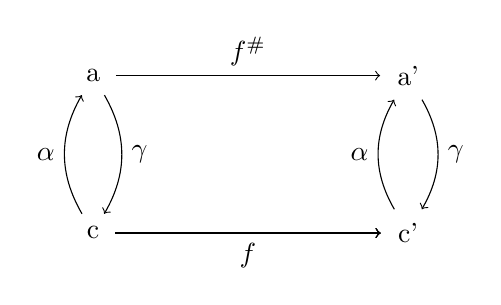
\begin{tikzpicture}
%            

         \node [circle] (A)  at (0,0)    {c};
  		 \node [circle] (B)  at (4,0)    {c'};
  		 \node [circle] (C)  at (0,2)    {a};
  		 \node [circle] (D)  at (4,2)    {a'};
  		 
  		 \draw [->] (A) --node[below]{$f$} (B); 
  		 \draw [->] (C) --node[above]{$f^\#$} (D); 
  		 \draw [->] (A) to [bend left=30] node[left]{$\alpha$}  (C); 
  		 \draw [->] (C) to [bend left=30] node[right]{$\gamma$} (A); 
  		 \draw [->] (B) to [bend left=30] node[left]{$\alpha$} (D); 
  		 \draw [->] (D) to [bend left=30] node[right]{$\gamma$} (B); 
  		 
  		 
  		 \draw [->] (A) -- (B); 
  		 \draw [->] (A) -- (B); 
  		 \draw [->] (A) -- (B); 
         
        \end{tikzpicture}
        \caption{The abstraction of a concrete function $f$.}\label{fig:abstractfunction}.
	\end{center}
\end{figure}